\chapter{Autonomous Search \& Autotuning}
\label{chap:autonomous}
\epigraph{\textit{There is nothing like looking, if you want to find something. You
certainly usually find something, if you look, but it is not always quite the
something you were after.}}{--- J.R.R. Tolkien, \textit{The Hobbit}}


\section{Algorithm Selection and Autonomous Solvers}
\label{sec:algselres}

In 1976 John R. Rice published \textit{The Algorithm Selection
Problem}~\cite{rice1976algorithm}, an influential paper where he formulated
abstract models for the problem of selecting effective algorithms for a given
problem. In Rice's framework the objective is to select the best algorithm,
according a performance metric, for a given problem. Consider a \textit{problem
space} $P$, and a problem $x \in P$.

Figure~\ref{fig:riceframe} presents Rice's algorithm selection
framework.
\todo[inline,author=Pedro,color=cyan]{Describe the framework in more detail}

\begin{figure}[htpb]
    \begin{center}
        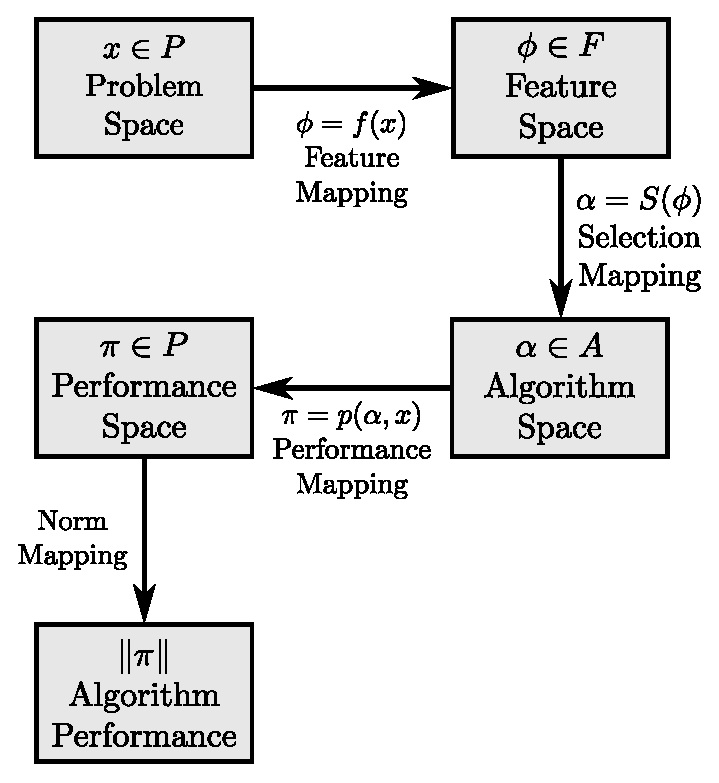
\includegraphics[width=.35\textwidth]{algorithm-selection}
    \end{center}
    \caption{Rice's framework}
    \label{fig:riceframe}
\end{figure}

\todo[inline,author=Pedro,color=cyan]{Discuss autonomous solvers}
\todo[inline,author=Pedro,color=cyan]{Discuss the choice of autotuning for
this work, given all the possibilities for solving the same problem
presented in this chapter}

\paragraph{On-line Control}
\label{sec:oncontrol}

% Final thesis should contain:
%
%\subsection{Adaptive Parameter Configuration}
%\label{subsec:paramadaptive}
%
%\subsection{Credit Assignment}
%\label{subsec:creditassign}
%
%\subsection{Reinforcement Learning}
%\label{subsec:reinforce}

\paragraph{Off-line Configuration}
\label{sec:offconfig}

% Final thesis should contain:
%\subsection{Evolutionary Computing}
%\label{subsec:evolcomp}
%
%\subsection{Stochastic Local Search}
%\label{subsec:searchsls}
%
%\subsection{Machine Learning}
%\label{subsec:searchml}

\section{Autotuning}
\label{sec:autotuning}

This section presents autotuning systems from different application domains,
categorized by the autotuning strategy they use. We gathered from the Google
Scholar bibliographic database the most relevant autotuning systems published
in the years of 2015, 2016 and 2017. We also discuss briefly notable autotuning
systems published before 2015.

The categories of autotuning strategies we use in this section are
\textit{Search Algorithms \& Heuristics}, \textit{Machine Learning \&
Model-Aided}, and \textit{Combinations}. Figure~\ref{fig:strategies} shows the
relations between the strategies. The intended contribution of this work is a
\textit{Domain-Agnostic System}, and we include this special category at the
end. Since we discuss the OpenTuner framework~\cite{ansel2014opentuner} in more
detail in this chapter, and we also use it in most case studies presented in
chapter~\ref{chap:usecases}, we also list autotuning systems that use it.

\begin{figure}[htpb]
    \centering
    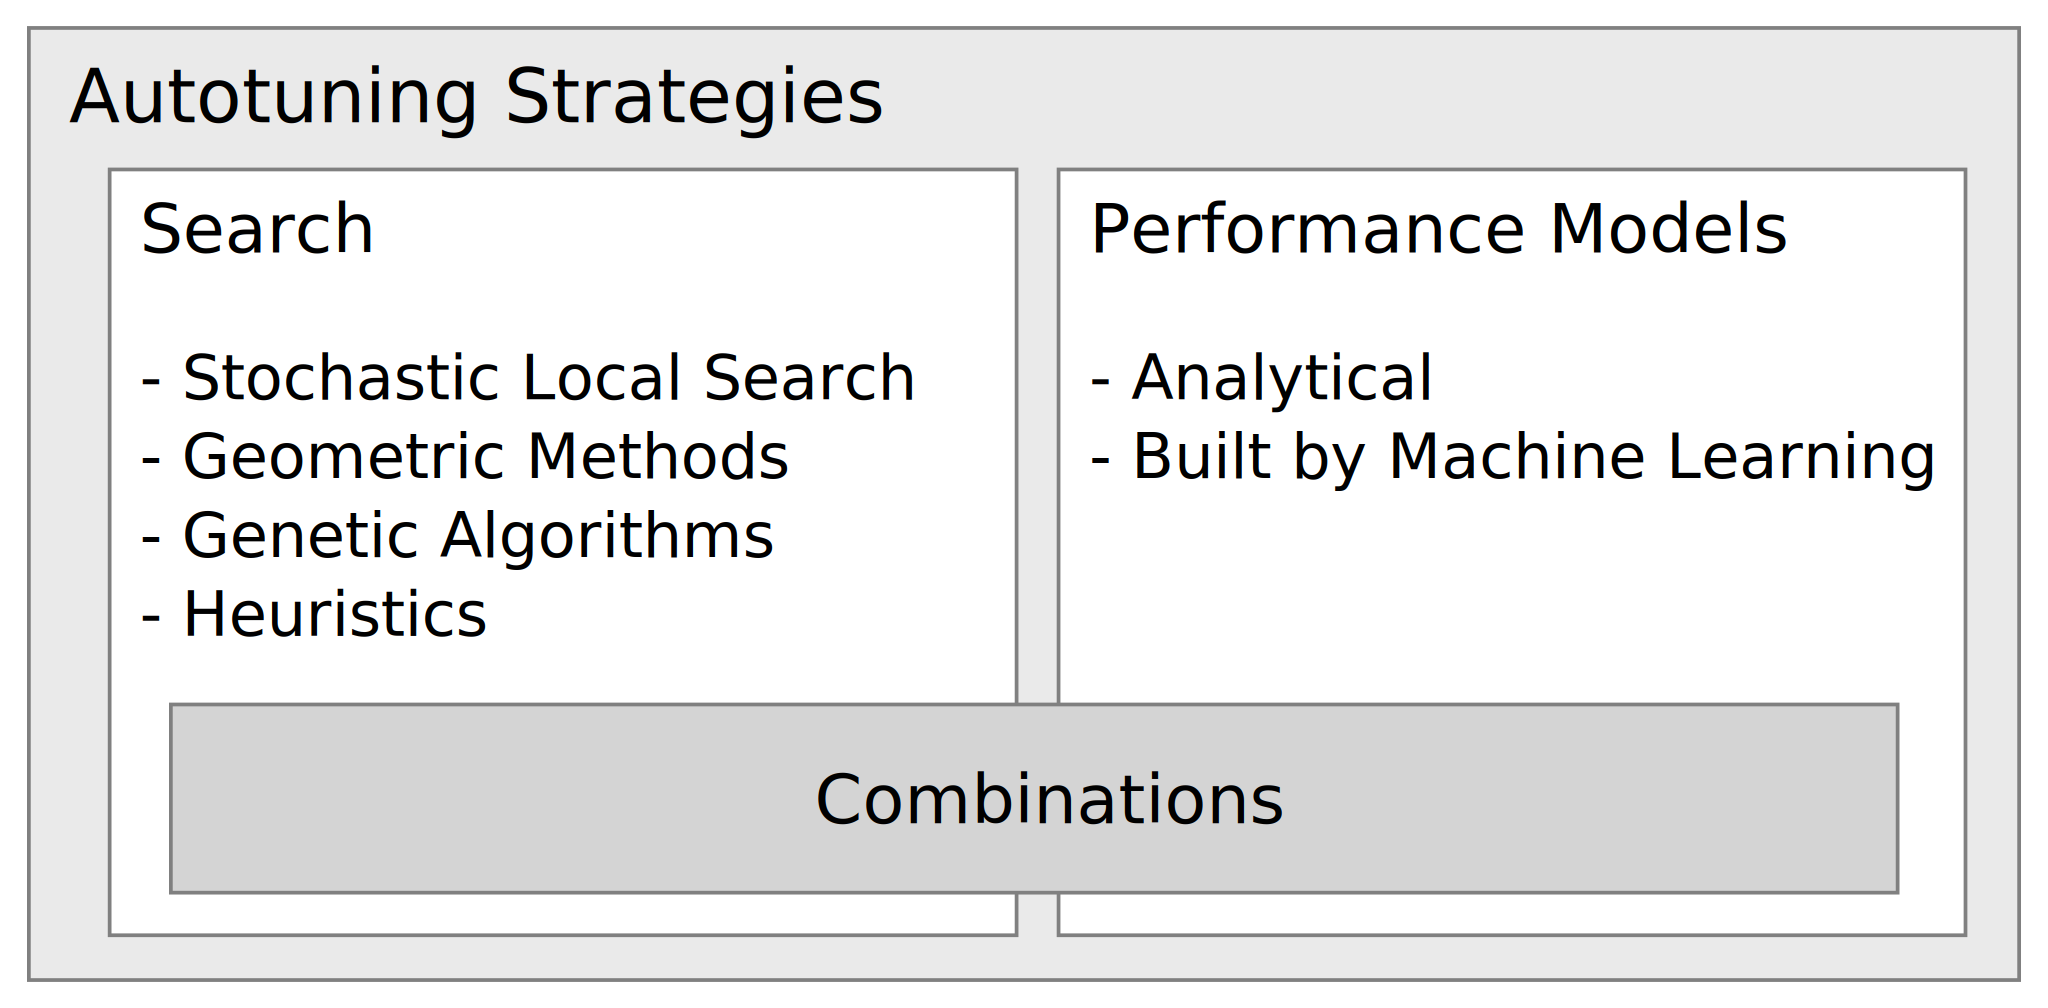
\includegraphics[width=.6\textwidth]{autotuning_strategies}
    \caption{Autotuning strategies discussed in this paper}
    \label{fig:strategies}
\end{figure}

Table~\ref{tab:systems} shows a selection of autotuning systems from different
problem domains, using different autotuning techniques. The variety of solutions
and domains makes clear that there is no single solution for all autotuning
problems, strengthening the argument that domain-agnostic autotuning systems
should use a combination of techniques when possible.

Rice's conceptual framework~\cite{rice1976algorithm} forms the foundation for
autotuners in various problem domains.  In 1997, the PHiPAC
system~\cite{bilmes1997optimizing} used code generators and search scripts to
automatically generate high performance code for matrix multiplication. Since
then, systems tackled different domains with a diversity of strategies. Whaley
\emph{et al.}~\cite{dongarra1998automatically} introduced the ATLAS project,
that optimizes dense matrix multiplication routines. The
OSKI~\cite{vuduc2005oski} library provides automatically tuned kernels for
sparse matrices. The FFTW~\cite{frigo1998fftw} library provides tuned C
subroutines for computing the Discrete Fourier Transform.

\begin{table}[htpb]
    \centering
    \begin{tabular}{@{}lll@{}}
        \toprule
        System & Domain & Technique \\ \midrule
        ATLAS~\cite{dongarra1998automatically} & Dense Linear Algebra & Exhaustive \\
        OSKI~\cite{vuduc2005oski} & Sparse Linear Algebra & Heuristic + Exhaustive \\
        LGen~\cite{spampinato2014basic} & Small-scale Linear Algebra & Exhaustive + Random \\
        INSIEME~\cite{jordan2012multi} & Compiler & Genetic Algorithm \\
        Petabricks~\cite{ansel2009petabricks} & Domain-Agnostic & Genetic Algorithm\\
        TANGRAM~\cite{chang2016efficient} & Heterogeneous Architectures & Breadth-First Search + Pruning \\
        Active Harmony~\cite{tapus2002active} & Runtime & Nelder-Mead \\
        MASE-BDI~\cite{coelho2016mase} & Environmental Land Change & Distributed Active Harmony~\cite{tapus2002active} \\
        ParamILS~\cite{hutter2009paramils} & Domain-Agnostic & Stochastic Local Search \\
        CLTune~\cite{nugteren2015cltune} & OpenCL kernels & Stochastic Local Search\\
        OPAL~\cite{audet2014optimization} & Domain-Agnostic & Direct Search \\
        MILEPOST GCC~\cite{fursin2011milepost} & Compiler & Central DB + Machine Learning \\
        Apollo~\cite{beckingsale2017apollo} & GPU kernels & Decision Trees \\
        OpenTuner~\cite{ansel2014opentuner} & Domain-Agnostic & Ensemble \\
        Periscope~\cite{gerndt2017multi} & HPC Applications & Various \\
        \bottomrule
    \end{tabular}
    \caption{Selected autotuning systems, their domains and techniques}
    \label{tab:systems}
\end{table}

\subsection{Search Algorithms \& Heuristics}

A common and still effective strategy for autotuning is to use search
algorithms, which can be simple such as simulated annealing and random walks,
or more elaborated, such as genetic algorithms and particle swarm optimization.
Search heuristics can also be developed and used effectively if an adequate
knowledge of the problem domain is obtained. When using search algorithms and
heuristics, autotuners must empirically evaluate program configurations to find
an optimized configuration. Most search algorithms and heuristics present few
or none convergence guarantees. Works in this category use search
algorithms and heuristics perform autotuning in different problem domains.

Abdelfattah \emph{et al.}~\cite{abdelfattah2016performance} present an
autotuning strategy using exhaustive evaluation of General Matrix-Matrix
Multiply (GEMM) kernel optimizations for GPUs. They later use this approach to
optimize GPU kernels for large-scale tensor
contractions~\cite{abdelfattah2016high}.  Guerreiro \emph{et
al.}~\cite{guerreiro2015multi} use search space pruning strategies and
exhaustive evaluation to autotune CUDA GPU kernels.
LGen~\cite{spampinato2014basic} is a compiler for small-scale linear algebra
computation that uses mathematical domain-specific languages to optimize loops
and vectorization. LGen uses exhaustive or random search to test different
optimizations.

Active Harmony~\cite{tapus2002active} provides an API that enables online
autotuning of a program using a variation of the Nelder-Mead simplex
algorithm~\cite{nelder1965simplex}.  MASE-BDI~\cite{coelho2016mase} is a
multi-agent system for the simulation of environmental land change that uses
the Active Harmony API~\cite{tapus2002active} and its search algorithms to
autotune  simulator parameters.  Several simulator configurations are executed
in parallel and communicate their results to a tuning manager using MPI.
CLTune~\cite{nugteren2015cltune} is an autotuning framework for OpenCL kernels
that uses search algorithms such as simulated annealing and particle swarm
optimization.  In an effort to provide a common representation of multiple
parallel programming models, the INSIEME compiler
project~\cite{jordan2012multi} implements abstractions for OpenMP, MPI and
OpenCL, and generates optimized parallel code for heterogeneous multi-core
architectures using genetic algorithms.

\subsection{Machine Learning \& Model-Aided}

Machine Learning algorithms have been used to solve an increasingly larger set
of Computer Science problems. The role of these algorithms in autotuners is to
build a performance model using a program's parameters, target architecture and
input.  The trained model can suggest new configurations for auxiliary search
algorithms or directly provide optimized configurations.

Tartara and Reghizzi~\cite{tartara2012parallel} use the MapReduce programming
model to improve the performance of machine learning algorithms in the
PetaBricks compiler. Later they presented a machine learning
algorithm~\cite{tartara2013continuous} that learns compiler heuristics using
data gathered after every compilation.  Mametjanov \emph{et
al.}~\cite{mametjanov2015autotuning} present an autotuning approach that uses
machine learning and selective sampling of the search space to optimize FPGA
hardware design parameters for performance and power.

Hou \emph{et al.}~\cite{hou2017auto} present an autotuning framework that uses
decision trees to optimize the sparse matrix-vector multiply kernel for multi
and many-core processors.  Apollo~\cite{beckingsale2017apollo} is an autotuning
framework for input-dependent kernels that uses a decision tree classifier that
provides optimizations that can be selected during runtime. MILEPOST
GCC~\cite{fursin2011milepost} and Collective Mind~\cite{fursin2015collective}
are notable research efforts in autotuning compiler optimizations.  These
projects build a central database of compiler optimizations and performance
metrics from collective experience and use machine learning algorithms to
improve autotuned suggestions.

Falsch and Elster~\cite{falch2017machine} build performance
models for OpenCL applications in different target architectures using machine
learning.  The learned statistical model is later used to pick promising
configurations for testing.  Balaprakash \emph{et
al.}~\cite{balaprakash2016automomml} introduce a framework that uses machine
learning algorithms to build models for metrics such as performance and energy
consumption, which are used for multi-objective optimization.

Autotuners can also use analytical performance models to suggest optimized
configurations.  Lang~\cite{lang2017data} reviews work on autotuning based on
analytical performance models, arguing that the approach is feasible.  Xu
\emph{et al.}~\cite{xu2016analytical} introduce an autotuning framework for
loop scheduling in GPUs that uses analytical performance models.
TuningGenie~\cite{ivanenko2014method} presents an autotuning framework that
uses code annotations and an analytical model for generating autotuners for
parallel programs.

\subsection{Combinations}

Systems in this category combine autotuning strategies from different
categories to improve found configurations and autotuner runtime.  The idea
behind a combination of autotuning techniques is that one strategy will
compensate the other. For example, the autotuner may detect that a random walk
algorithm got stuck in a local minima of the search space, in which point the
autotuner could start using a hill-climbing algorithm.

Garvey \emph{et al.}~\cite{garvey2015automatic} present a strategy to autotune
OpenCL GPU kernels using machine learning, heuristics for search space
partitioning and exhaustive search.  PolyMage~\cite{mullapudi2015polymage} is a
domain-specific language and compiler for image processing pipelines. It uses
heuristics and performance models to prune the search space, which is then
explored exhaustively.  Ziegler \emph{et
al.}~\cite{ziegler2016synthesis,ziegler2016scalable} present an autotuning
system for hardware synthesis parameters that uses genetic and learning
algorithms to explore the hardware design space for real industrial chip
designs from IBM.  Ngoko \emph{et al.}~\cite{ngoko2016automatic} introduce an
autotuning system for $\NP$-hard problems that uses distributed measurements of
configurations and machine learning algorithms aided by randomization,
clustering and set intersection solvers.  Luo \emph{et al.}~\cite{luo2015fast}
present a framework for stencil computations that uses Optimal-Solution Spaces,
input feature extraction and machine learning.

\subsection{Domain-Agnostic Systems}

In this work the Domain-Agnostic category refers to autotuners that provide
general abstractions for the representation of search spaces from different
problem domains. These abstractions are used to represent program parameters
and configurations and enable the implementation of autotuners for various
problem domains. Domain-Agnostic systems must also employ a robust set of
autotuning techniques in order to achieve good performance in different
domains.

Petabricks~\cite{ansel2009petabricks} is a language and compiler that enables
the expression of program implementation search spaces at language level.
OpenTuner~\cite{ansel2014opentuner} is a domain-agnostic autotuning framework
that provides ensembles of search techniques for user-defined program
configurations.  The ParamILS framework~\cite{hutter2009paramils} applies
stochastic local search methods for algorithm configuration and parameter
tuning.  TANGRAM~\cite{chang2015tangram,chang2016efficient} is a kernel
synthesis framework for different architecture hierarchies.  It uses
composition rules and breadth-first search to prune and explore the design
space.  The Periscope Tuning Framework
(PTF)~\cite{gerndt2005periscope,gerndt2010automatic,gerndt2017multi} is an
online tool for performance analysis and tuning that has a modular architecture
based on plugins.  OPAL~\cite{audet2014optimization} is domain-agnostic system
for parameter optimization that uses direct search and is able to run parallel
and distributed measurements.

\subsubsection{Works using OpenTuner}

Since the publication of the OpenTuner in 2014, work in different domains
validated the framework's efficacy in implementing autotuners. Most case
studies we present in chapter~\ref{chap:usecases} also used OpenTuner.

Takizawa \emph{et al.}~\cite{takizawa2017customizable} use
OpenTuner~\cite{ansel2014opentuner} and Xevolver~\cite{takizawa2014xevolver}, a
code transformation framework, to enable the autotuning of code transformations
in applications that were not implemented for autotuning. They present an
autotuning ``scenario template'' that uses compiler directives to inform the
autotuner.  Bosboom \emph{et al.} and Eliahu use OpenTuner to implement a
domain specific language for data-flow programming~\cite{bosboom2014streamjit}
and a framework for recursive parallel algorithm
optimization~\cite{eliahu2015frpa}.

Xu \emph{et al.}~\cite{xu2017parallel} present an autotuning strategy that uses
parallel OpenTuner instances to autotune the FPGA compilation flow.  Their work
dynamically partition the search space between MPI-communicating OpenTuner
instances.  Jayasena \emph{et al.}~\cite{jayasena2015auto} use OpenTuner to
implement an autotuner for a Java Virtual Machine implementation.

\section{The OpenTuner Framework}
\label{sec:opentuner}
\todo[inline,author=Pedro,color=cyan]{This section will describe OpenTuner in
more detail}

\subsection{Software Architecture}
\label{sec:arch}
\todo[inline,author=Pedro,color=cyan]{Describe OpenTuner architecture and the
dependent execution flow of measurement and search}

\subsection{Search Techniques}
\label{sec:techniques}
\todo[inline,author=Pedro,color=cyan]{Describe search techniques and MAB}

\subsection{Parallel and Distributed Programming in OpenTuner}
\label{sec:opentuner-parallel}
\todo[inline,author=Pedro,color=cyan]{Discuss OpenTuner's limitations and shortcomings.}
\todo[inline,author=Pedro,color=cyan]{Discuss the difficulties and
explain why they motivated the new Julia code.}

% Final thesis should contain:
%
%\subsection{Benchmarks}
%\label{sec:benchmarks}
%
%\subsubsection{Solvers of NP-Complete Problems}
%\label{subsec:np}
%
%\subsubsection{Algorithm Selection and Configuration}
%\label{subsec:algsel}
%
%\subsubsection{Compiler Configuration}
%\label{subsec:compilerconfig}
%
%\subsubsection{Measurement Time}
%\label{subsec:measure}
